\section{State of the Art}

\subsection{Depth perception}

Obtaining depth perception data from an image sensor can be a daunting
task, due to the nature of the media used in the process. In order to be 
able to assess  2-dimensional image from a 3-dimensional perspective, the
best example that can be used is human vision. While cameras operate in a
similar fashion to our eyes, with light information being converted into 
electrical impulses, the difference in understanding 3-dimensional space
comes from our ability to interpret several visual cues that we associate 
with a difference in depth.

Those cues can relate to the relative positioning of the objects within a 
given scene (occlusion and size difference), their appearance (atmospheric
perspective and texture gradient), the dynamic of the scene (motion parallax),
or the perspective of the viewer (convergence and stereopsis)~\cite{withGeneralDepth}.

For the case of occlusion and size difference, although the importance of the cues
are relevant for humans due to their experience, programming them into an autonomous
system could lead to potential false positive results, such as the following case:

\begin{figure}[H]
    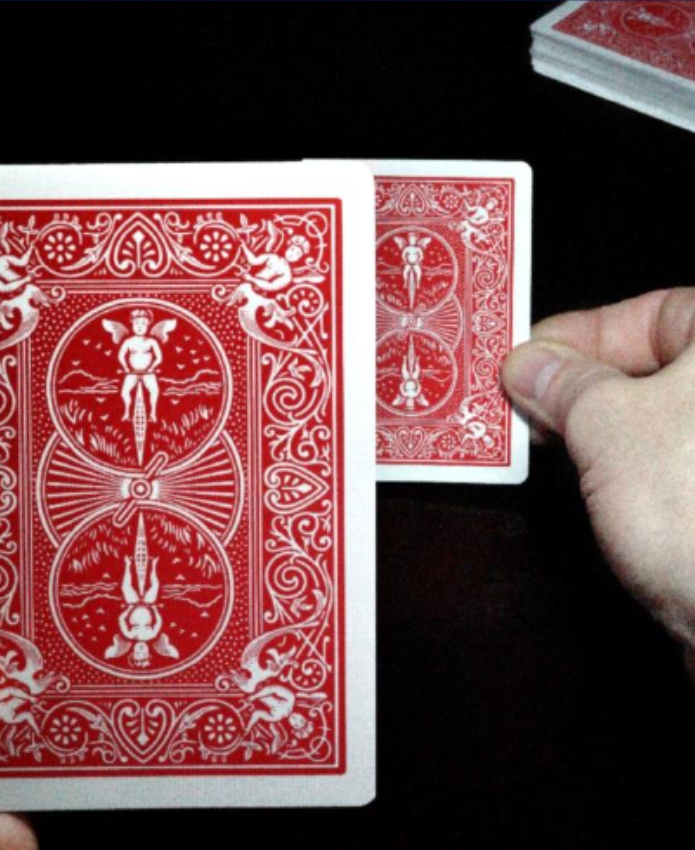
\includegraphics[width=0.35\textwidth, height=0.35\textwidth]{resources/png/occlusion_mislead.png}
    \caption{Occlusion mislead.~\cite{withGeneralDepth}~\label{figMislead}}
\end{figure}

In order to make use of atmospheric perspective, the scene depth needs to be in the
order of kilometers, such as the following:

\begin{figure}[H]
    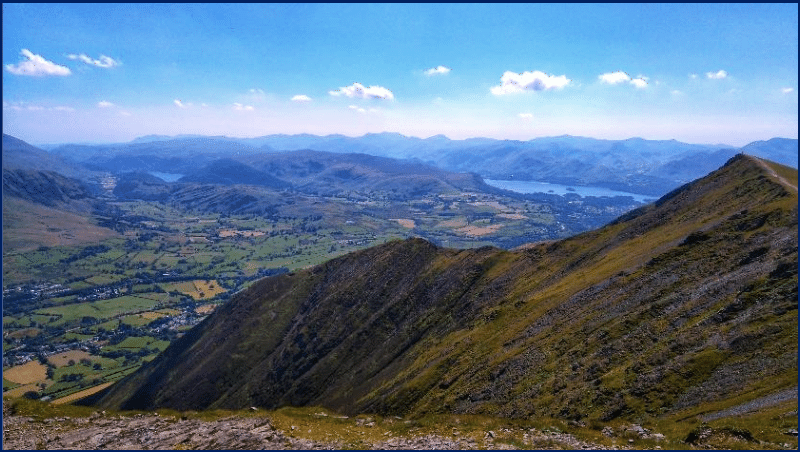
\includegraphics[width=0.75\textwidth, height=0.25\textwidth]{resources/png/atmospheric_perspective.png}
    \caption{Atmospheric perspective.~\cite{withGeneralDepth}~\label{figAtmos}}
\end{figure}

and for the texture gradient to be relevant it needs to be readily noticeable:

\begin{figure}[H]
    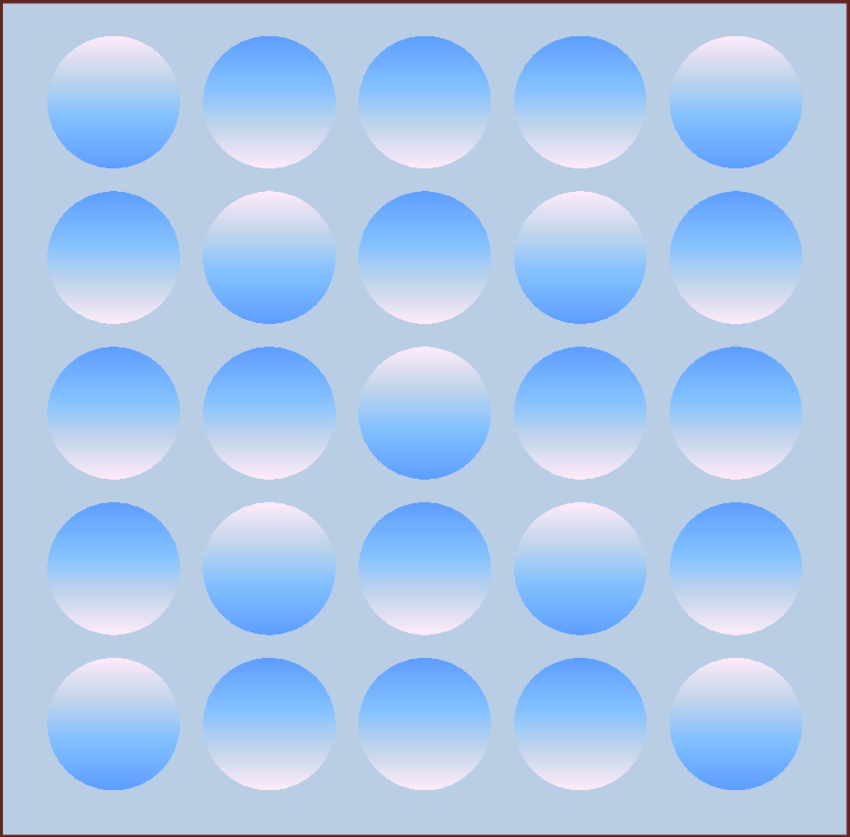
\includegraphics[width=0.25\textwidth, height=0.25\textwidth]{resources/png/texture.png}
    \caption{Texture gradient.~\cite{withGeneralDepth}~\label{figTexture}}
\end{figure}

Thus, in order to make use of those two cues, the scene composition needs to be curated
accordingly, ruling out broader applications.

Motion parallax refers to the difference in perceived motion, based on the proximity 
to the viewer. Closer entities appear to be moving faster, in relation to background 
objects that seem slower or even still, depending on the distance to the camera. In 
the case of still images, this phenomenon manifests as different degrees of blur, 
depending on the velocity of each object~\cite{withGeneralDepth}:

\begin{figure}[H]
    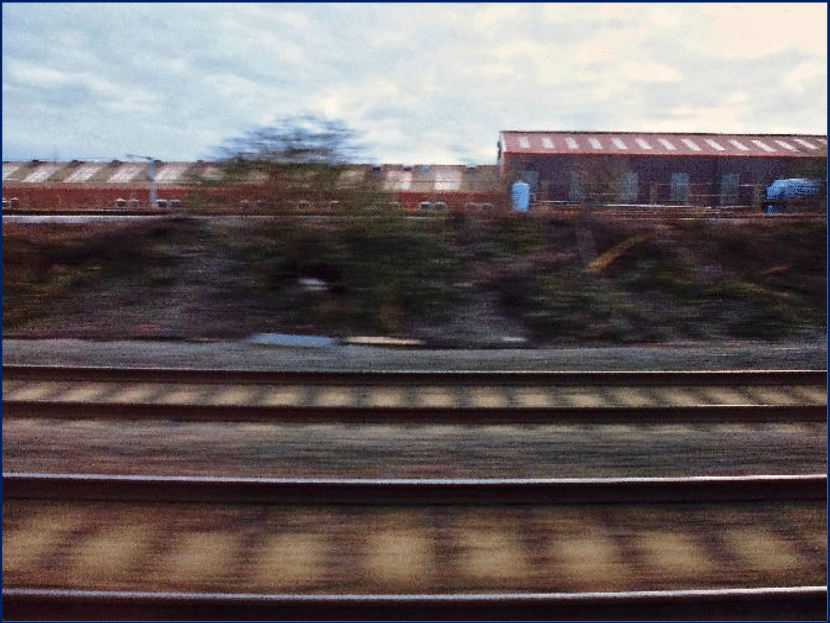
\includegraphics[width=0.75\textwidth, height=0.25\textwidth]{resources/png/parallax.png}
    \caption{Parallax effect.~\cite{withGeneralDepth}~\label{figParallax}}
\end{figure}

While the blur could be quantized in order to obtain image depth, the use cases are
again fringe, as the scene needs to be dynamic.

Used by architects and artists alike, perspective convergence refers to the use of 
converging lines in order to denote the depth of a scene. This leads to convergence
being a relevant clue in most cases, as perspective line can be derived from the
scene composition:

\begin{figure}[H]
    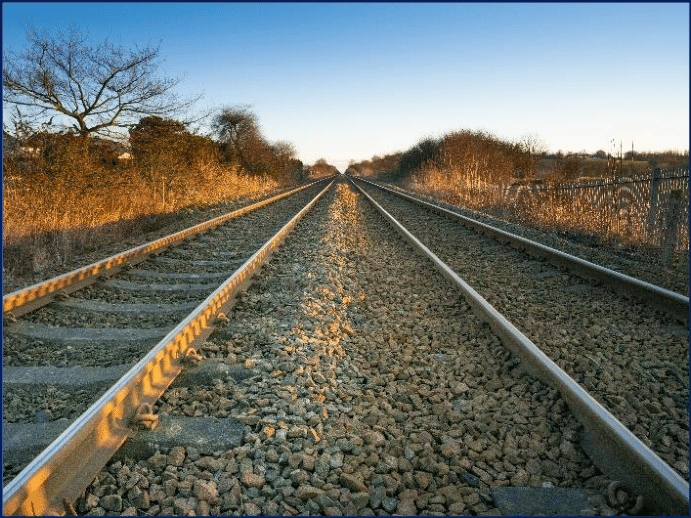
\includegraphics[width=0.50\textwidth, height=0.25\textwidth]{resources/png/convergenceGood.png}
    \caption{Convergence.~\cite{withGeneralDepth}~\label{figGood}}
\end{figure}

However, convergence can interfere with the interpretation of other cues, such as 
size difference, leading to optical illusions~\cite{withGeneralDepth}:

\begin{figure}[H]
    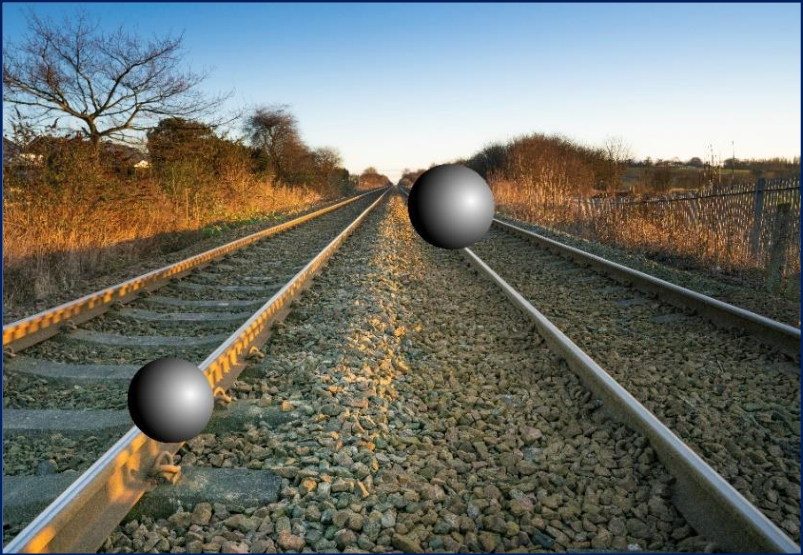
\includegraphics[width=0.50\textwidth, height=0.25\textwidth]{resources/png/convergenceBad.png}
    \caption{Convergence and size illusion.~\cite{withGeneralDepth}~\label{figBad}}
\end{figure}

This leads to stereopsis as the sole viable candidate for depth perception,
as it relies on the comparison of two slightly different images, with the disparity
between them being interpreted as 3-dimensional cues~\cite{withGeneralDepth}:

\begin{figure}[H]
    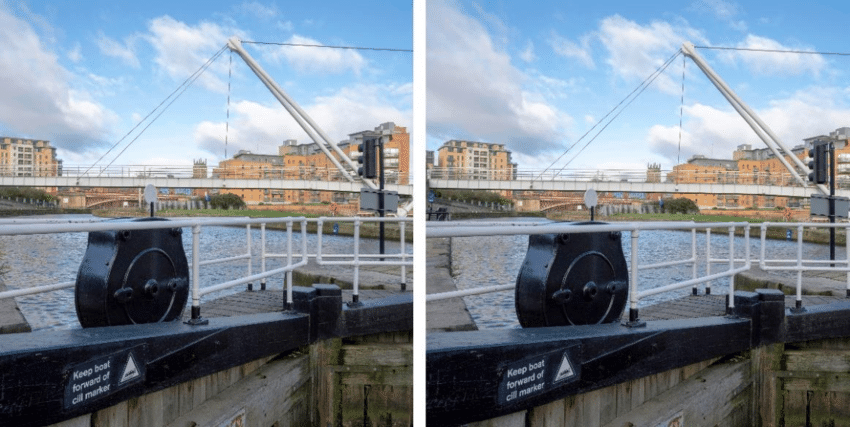
\includegraphics[width=0.50\textwidth, height=0.25\textwidth]{resources/png/stereopsis.png}
    \caption{Stereopsis.~\cite{withGeneralDepth}~\label{figStereo}}
\end{figure}

While it may not be reliable for cases where image depth is so great that the disparity
becomes irrelevant, stereopsis can provide valid data for a myriad of applications,
and at the same time be easily implementable as an embedded system, through the use of
separate image sensors with a common control module, similar in may ways to human vision.

\subsection{Stereo vision}

As it is cumbersome to extract 3-dimensional information from a monocular perspective without
specialized artificial intelligence tools~\cite{withAI}, as well as the same perspective leading
to different results on different cameras, stereopsis became one of the most popular methods
for depth perception.~\cite{withApplications}

The baseline principle for stereo vision is ``epipolar geometry'', relying on the input of two
cameras with different positions observing the same scene, resulting in two separate perspectives
of the same subject. Under those conditions, ``epipolar lines'' can be derived from the analysis
of a certain point in space and its projections onto the two images~cite{withApplications}:

\begin{figure}[H]
    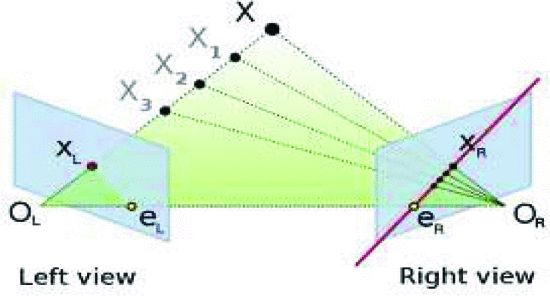
\includegraphics[width=0.50\textwidth, height=0.25\textwidth]{resources/png/epipolar_geometry.png}
    \caption{Epipolar geometry.~\cite{withApplications}~\label{figEpipolar}}
\end{figure}

In the case above, the ``epipolar lines are a function of the 3D point X, and for every 3D point,
there is a set of epipolar lines in both images''. \(O_{L}\) and \(O_{R}\) represent the center of
projection for each of the cameras, with \(X_{L}\) and \(X_{R}\) respectively being the image
points corresponding to \(X\). The projection of each center onto the other camera's image 
represent the ``epipolar points'', \(e{L}\) and \(e_{R}\), and they are aligned with the centers
of projection on a 3-dimensional line, outside of the images. Due to the alignment of points 
\(O_{L}\), \(X_{L}\) and \(X\), the representation of the line \(O_{L} - X_{L}\) onto the left 
image is a single point, while in the right images plane it is observed as the epipolar line
\(e_{R} - X_{R}\). The opposite also holds true, with the line \(O_{R} - X_{R}\) corresponding
to the epipolar line \(e_{L} - X_{L}\)~\cite{withApplications}.

Due to those properties, the following observations can be made, as long as ``the relative 
translation and rotation of the two cameras is known'':
\begin{itemize}
    \item If the projection point \(X_{L}\) is known, then the epipolar line \(e_{R} - X_{R}\)
is also known.
    \item If both projection points \(X_{L}\) and \(X_{R}\) are known, then their projection lines
are also known.
\end{itemize}

Those observations provide ``epipolar constraints'', allowing for the check of corresponding points
in order to determine wether or not they represent the same spatial point. They also allow for the
triangulation of the 3-dimensional point, as long as both its projections are known. Using those
principles, image depth can be calculated using the disparity between scenes captured by different
cameras~\cite{withApplications}.

\begin{figure}[H]
    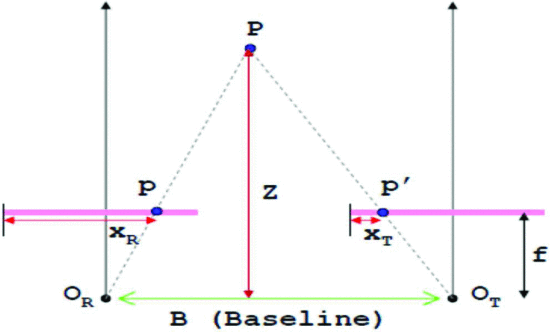
\includegraphics[width=0.50\textwidth, height=0.25\textwidth]{resources/png/depth_calculation.png}
    \caption{Depth calculation.~\cite{withApplications}~\label{figDepthCalc}}
\end{figure}

Disparity refers to ``the relative shift between two matching pixels'', and scales inversely 
proportional to the depth, meaning that points closer to the camera will be more shifted than
those further away.  In the case of~\ref{figDepthCalc}
the depth can be calculated using epipolar geometry, with the left image being used as a reference,
and the right one as the target image. Points \(O_{R}\) and \(O_{T}\) the optical 
centers of each camera, \(P\) the target point in the scene, and \(X_{R}\) and \(X_{T}\)
representing the relative coordinates of the projection points \(p\) and \(p'\), using the
following relations~\cite{withApplications}:
\begin{equation}
    \frac{Z}{Z-f} = \frac{B}{(B + X_{T} - X_{R})}
\end{equation}

\begin{equation}
    Z = \frac{B \times f}{X_{R} - X{T}}
\end{equation}

\begin{equation}
    Z = \frac{B \times f}{d}
\end{equation}

where \(d\) denotes the disparity \(X_{R} - X_{T}\), \(z\) represents the depth, with coefficients 
\(B\) and \(F\) denoting the distance between the cameras, and the focal lengths, respectively.

As an additional step that reduces scene clutter, an edge detection filter, such as Sobel or Canny 
is applied. This step leaves in the scene only those points that are relevant for the disparity 
calculation.

The final step is the ``depth map generation'', in which the disparity between all corresponding pixels
is computed and stored into a matrix, holding the relative depth of each pixel as a grey scale value.
~\cite{withApplications}

\begin{figure}[H]
    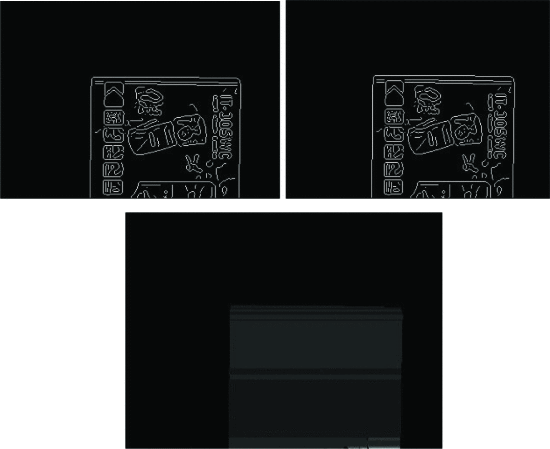
\includegraphics[width=0.50\textwidth, height=0.45\textwidth]{resources/png/depth_map.png}
    \caption{Canny filter and depth map.~\cite{withApplications}~\label{figDepthMap}}
\end{figure}

\subsubsection{Applications}

In practice, this process is used for tasks that require precise data about the distance from the 
viewer to the points in the scene. The most prominent case of such a use case is autonomous driving,
due to the myriad of potential hazards surrounding an unmanned vehicle.

In the particular case of an ``Autonomous Surface Vehicle (ASV)'', the proposed solution relies on the
coordination between stereoscopic inputs, as well as a GPS signal. The system has the following hardware
architecture~\cite{withNavigation}:

\begin{figure}[H]
    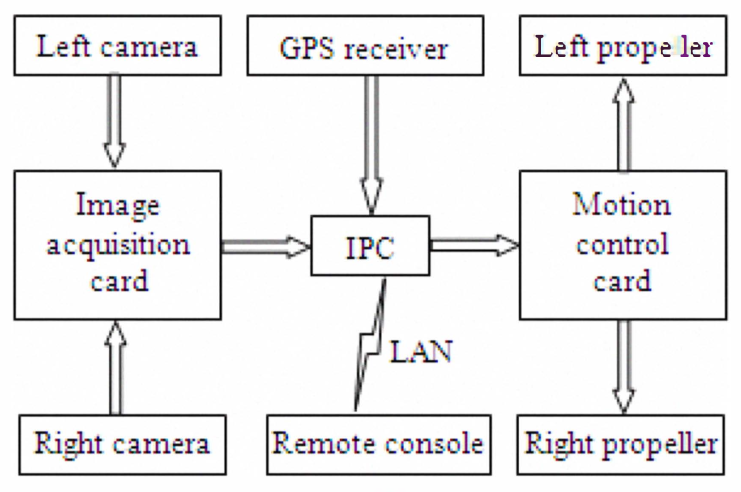
\includegraphics[width=0.75\textwidth, height=0.35\textwidth]{resources/png/boat_architecture.png}
    \caption{ASV hardware architecture.~\cite{withNavigation}~\label{figNav}}
\end{figure}

The images provided by the cameras are fed into an image processing module, where several filtering steps
are carried out, before the relevant features are extracted and used to create the disparity map. From 
there, the camera parameters are taken into account, and the position and distance of potential obstacles
are computed. This information is passed to a path finding algorithm that determines the adequate control
signal for each propeller.

Another implementation improves upon the initial algorithm, increasing its reliability such that it could
be used for fast obstacle detection on the road. The most relevant addition is an ``adaptive thresholding
scheme'', used to reduce the amount of noise that can affect data from the furthest points in the scene.
Additionally, two enhancement steps are taken, both for the horizontal as well as the vertical disparity
maps, in order to correctly assess wether a group of pixels is an obstacle.~\cite{withMain}

In the case of vertical enhancement, the disparity map is scanned both top-down and bottom-up, with 
pixels that are determined to be part of an obstacle generating a scan of their neighborhood, and any
other pixels of similar disparity being considered as part of the same obstacle. For horizontal 
enhancement, the disparity map is scanned row by row, with the maximum being recorded and used to 
analyze the following row. Those maximums are then used to generate the ``road profile'', based on the
assumption that obstacle pixels have a higher disparity then road pixels.~\cite{withMain}

\begin{figure}[H]
    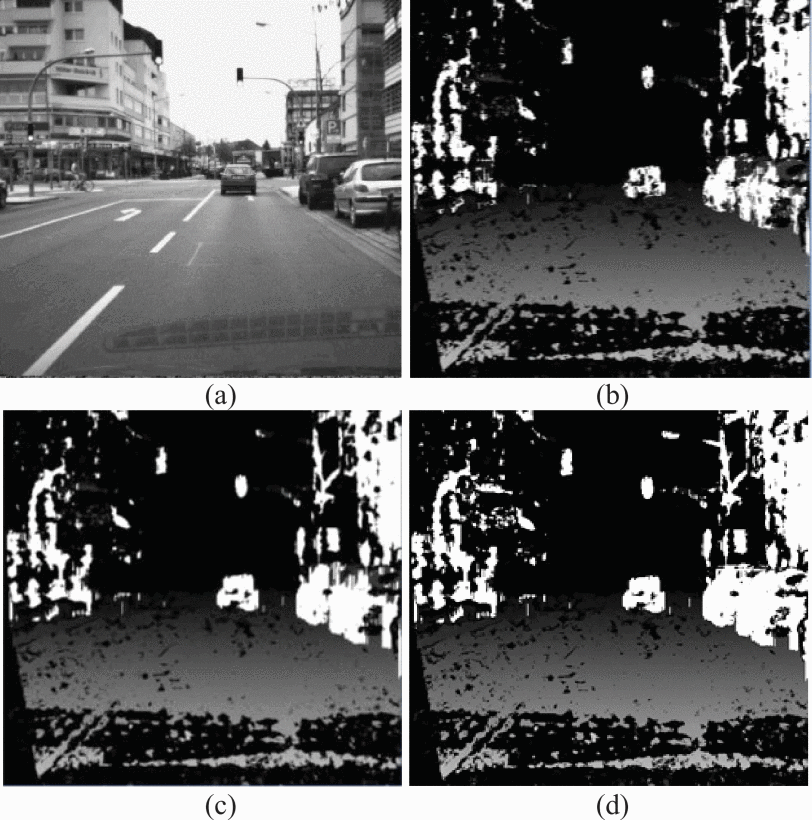
\includegraphics[width=0.50\textwidth, height=0.45\textwidth]{resources/png/final_result.png}
    \caption{Processing steps.~\cite{withMain}~\label{figSteps}}
\end{figure}

\subsection{Multiple view stereopsis}

Also taking inspiration from nature, this time however from the way insects perceive their
environment, micro-lens arrays focus light in several spots of the image sensor. Through this,
several similar images are created, and those disparities can be analyzed in order to assess
the depth of the scene, similar to stereo vision systems.

The design is based on the study of ``Xenos pekii'', insects that are capable of ``multi-view
stereopsis with high visual acuity through chunk sampled images, which is created by multiple 
photoreceptors on a single facet lens''. Similarly, ``multi-aperture systems'' are capable of
capturing a series of perspective scenes around the same target object, all in a singe shot.
~\cite{withInsects}

Although there are limitations in recreating the visual patterns of a Xenos pekii with traditionally
flat image sensors, the ``ultrathin microlens array camera (MAC)'' aims to emulate the insect view
through the use of ``constant FOV microlens arrays''. The lens array allows for the capture of
``partial images with all-in-focus'', allowing for more accurate disparity calculations.
~\cite{withInsects}

\begin{figure}[H]
    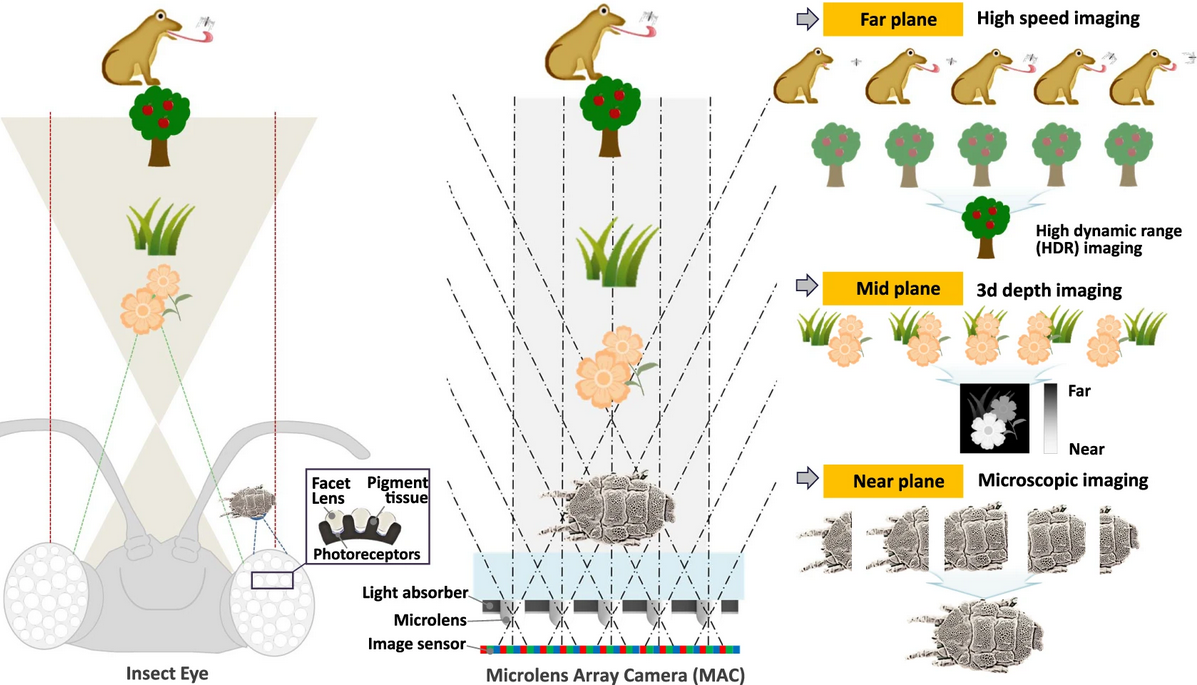
\includegraphics[width=0.75\textwidth, height=0.35\textwidth]{resources/png/paper_working.png}
    \caption{Parallel between insect stereopsis and MAC.~\cite{withInsects}~\label{figInsects}}
\end{figure}

\subsection{Curved image sensor}

The idea originates from the need for ``soft biometric devices'', meant to act as implantable devices
meant to assist with diminishing organ functions, in this case those of the retina. Several such image
sensor arrays were proposed, among which is the ``hemispherically curved image sensor (CurvIS)'', that
can achieve ``aberration-free imaging and a wide field-of-view''. Its design is based on ``ultrathin
\(MoS_{2}\)'', a novel 2-dimensional nanomaterial, whose advantages are its ``superb photo-absorption
coefficient, photoresponsivity, and high fracture strain''.~\cite{withHexagons}

\begin{figure}[H]
    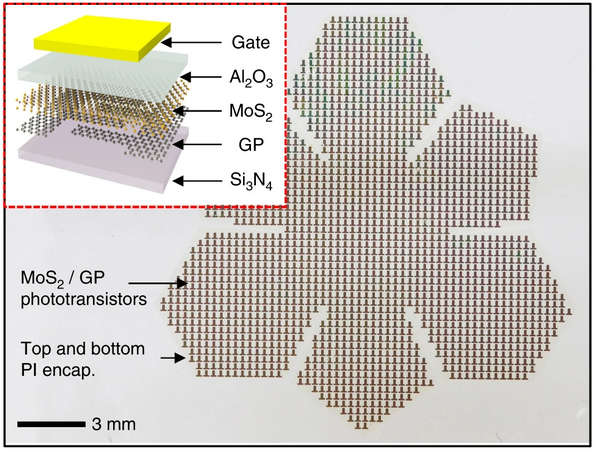
\includegraphics[width=0.55\textwidth, height=0.45\textwidth]{resources/png/paper_sensor.png}
    \caption{Proposed truncated icosahedron design for phototransistor array.~\cite{withHexagons}~\label{figSensor}}
\end{figure}

Due to the requirement for the hemispherical construction of the image sensor, the use of a classical 
``film-type image sensor array'' is inadequate, due to the mechanical strain that could induce failures
in the device. Thus, the sensor is composed of a ``\(MoS_{2}\)-graphene heterostructure'' as well as other
sublayers, leading to a final device thickness of ``\(51nm\)'', thicker than the average silicon-based 
sensor, but with significantly greater fracture strain and higher photo-absorption coefficient.